\documentclass[10pt, aspectratio=169, xcolor={dvipsnames}]{beamer}

% --- Theme ---
\usetheme{metropolis}
\usepackage[utf8]{inputenc}
\usepackage[english]{babel}
\usepackage{amsmath, amsfonts, amssymb}
\usepackage{tikz}
\usetikzlibrary{arrows.meta, shapes.geometric, positioning, decorations.pathreplacing, calc}
\usepackage{pgfplots}
\usepackage{booktabs}
\usepackage{xcolor}
\usepackage{graphicx}
\usepackage{animate}
\usepackage{multimedia}

\pgfplotsset{compat=1.18}

% --- Custom colours ---
\definecolor{gaussblue}{RGB}{30, 100, 180}
\definecolor{accentorange}{RGB}{230, 100, 20}
\definecolor{softgreen}{RGB}{34, 139, 34}
\definecolor{lightgray}{RGB}{240, 240, 240}
\setbeamercolor{alerted text}{fg=accentorange}
\setbeamercolor{example text}{fg=softgreen}

% --- Metadata ---
\title{3D Gaussian Splatting}
\subtitle{Real-time Rendering and SLAM}
\author{Jaime Hernández \and Yauheni Yatsevich}
\institute{Universidad de Alicante}
\date{March 2026}

\begin{document}

% ============================================================
% SLIDE 1 — Title
% ============================================================
\begin{frame}
  \titlepage
\end{frame}

% ============================================================
% SLIDE 2 — The Problem
% ============================================================
\begin{frame}{The Goal: See the World from Any Angle}
  \begin{columns}[c]
    \begin{column}{0.42\textwidth}
      \textbf{Can a computer reconstruct a 3D scene just from photos?}

      \vspace{0.7em}
      \begin{enumerate}
        \item Take photos from multiple angles
        \item Build a 3D model
        \item Render from \alert{any new viewpoint} — in real time
      \end{enumerate}

      \vspace{0.7em}
      \begin{exampleblock}{Applications}
        VR/AR · Film VFX · Robotics · Digital heritage
      \end{exampleblock}
    \end{column}
    \begin{column}{0.56\textwidth}
      \centering
      % Visual: cameras around an object → novel view
      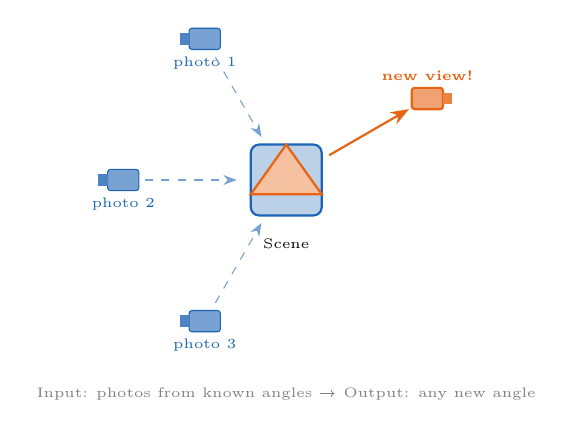
\begin{tikzpicture}[scale=0.9]
        % Central object (scene)
        \fill[gaussblue!30, draw=gaussblue, thick, rounded corners=3pt]
          (-0.5,-0.5) rectangle (0.5,0.5);
        \fill[accentorange!40, draw=accentorange, thick]
          (0,0.5) -- (0.5,-0.2) -- (-0.5,-0.2) -- cycle;
        \node[font=\tiny, below] at (0,-0.7) {Scene};

        % Cameras around (input)
        \foreach \angle/\n in {120/1, 180/2, 240/3}{
          \begin{scope}[shift={({2.3*cos(\angle)},{2.3*sin(\angle)})}]
            \fill[gaussblue!60, draw=gaussblue, rounded corners=1pt]
              (-0.22,-0.15) rectangle (0.22,0.15);
            \fill[gaussblue!80] (-0.22,-0.08) rectangle (-0.35,0.08);
            \node[font=\tiny, gaussblue, below=3pt] {photo \n};
          \end{scope}
          \draw[-{Stealth}, gaussblue!60, dashed]
            ({2.0*cos(\angle)},{2.0*sin(\angle)}) -- ({0.7*cos(\angle)},{0.7*sin(\angle)});
        }

        % Novel view (output)
        \begin{scope}[shift={({2.3*cos(30)},{2.3*sin(30)})}]
          \fill[accentorange!60, draw=accentorange, thick, rounded corners=1pt]
            (-0.22,-0.15) rectangle (0.22,0.15);
          \fill[accentorange!80] (0.22,-0.08) rectangle (0.35,0.08);
          \node[font=\tiny, accentorange, above=3pt] {\textbf{new view!}};
        \end{scope}
        \draw[-{Stealth}, accentorange, thick]
          ({0.7*cos(30)},{0.7*sin(30)}) -- ({2.0*cos(30)},{2.0*sin(30)});

        \node[font=\tiny, gray, below] at (0,-2.8) {Input: photos from known angles → Output: any new angle};
      \end{tikzpicture}
    \end{column}
  \end{columns}
\end{frame}

% ============================================================
% SLIDE 3 — Two approaches
% ============================================================
\begin{frame}{Two Approaches to the Same Problem}
  \begin{columns}[c]

    \begin{column}{0.5\textwidth}
      \centering
      \textbf{\color{gaussblue} NeRF} — \emph{"Neural" approach}

      \vspace{0.4em}
      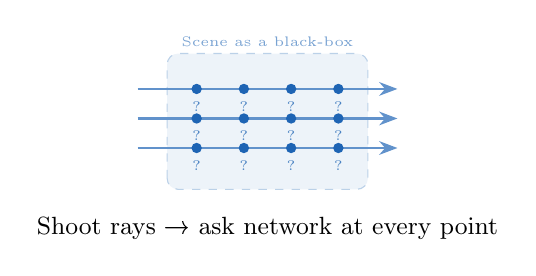
\begin{tikzpicture}[scale=0.75]
        % Scene volume
        \fill[gaussblue!8, draw=gaussblue!30, dashed, rounded corners=4pt]
          (-1.7,-0.3) rectangle (1.7,2.0);
        \node[font=\tiny, gaussblue!60] at (0,2.2) {Scene as a black-box};
        % Rays
        \foreach \y in {0.4, 0.9, 1.4}{
          \draw[-{Stealth}, gaussblue!70, thick] (-2.2,\y) -- (2.2,\y);
          \foreach \x in {-1.2, -0.4, 0.4, 1.2}{
            \fill[gaussblue] (\x,\y) circle (2.5pt);
            \node[font=\tiny, gaussblue!80, below=1pt] at (\x,\y) {?};
          }
        }
        \node[below, font=\small] at (0,-0.6) {Shoot rays → ask network at every point};
      \end{tikzpicture}

      \vspace{0.3em}
      \begin{alertblock}{\centering Bottleneck}
        \centering Thousands of neural-network queries \textbf{per pixel}\\
        Training: 1–2 days \quad Speed: $<$1 FPS
      \end{alertblock}
    \end{column}

    \begin{column}{0.5\textwidth}
      \centering
      \textbf{\color{accentorange} 3D Gaussian Splatting} — \emph{"Explicit" approach}

      \vspace{0.4em}
      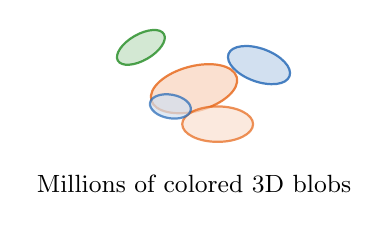
\begin{tikzpicture}[scale=0.75]
        % Gaussians scattered
        \begin{scope}[rotate around={15:(0,0.8)}]
          \draw[accentorange, thick, fill=accentorange!25, opacity=0.8] (0,0.8) ellipse (0.75cm and 0.38cm); \end{scope}
        \begin{scope}[rotate around={-20:(1.1,1.2)}]
          \draw[gaussblue, thick, fill=gaussblue!25, opacity=0.8] (1.1,1.2) ellipse (0.55cm and 0.28cm); \end{scope}
        \begin{scope}[rotate around={30:(-0.9,1.5)}]
          \draw[softgreen, thick, fill=softgreen!25, opacity=0.8] (-0.9,1.5) ellipse (0.45cm and 0.22cm); \end{scope}
        \begin{scope}[rotate around={0:(0.4,0.2)}]
          \draw[accentorange, thick, fill=accentorange!20, opacity=0.7] (0.4,0.2) ellipse (0.60cm and 0.30cm); \end{scope}
        \begin{scope}[rotate around={-10:(-0.4,0.5)}]
          \draw[gaussblue, thick, fill=gaussblue!20, opacity=0.7] (-0.4,0.5) ellipse (0.35cm and 0.20cm); \end{scope}
        \node[below, font=\small] at (0,-0.5) {Millions of colored 3D blobs};
      \end{tikzpicture}

      \vspace{0.3em}
      \begin{exampleblock}{\centering Result}
        \centering Just \textbf{project blobs} onto screen (GPU-fast)\\
        Training: 20–40 min \quad Speed: \textbf{$>$90 FPS}
      \end{exampleblock}
    \end{column}
  \end{columns}
\end{frame}

% ============================================================
% SLIDE 3b — Visual comparison COLMAP / NeRF / 3DGS
% ============================================================
\begin{frame}{Comparison: COLMAP → NeRF → 3DGS}
  \centering
  \animategraphics[loop, autoplay, width=0.92\textwidth]{12}{images/gifs/compare_frames/frame-}{000}{080}

  \vspace{0.4em}
  \begin{columns}[c]
    \begin{column}{0.32\textwidth}
      \begin{block}{\centering COLMAP}
        \centering Sparse point cloud from photos
      \end{block}
    \end{column}
    \begin{column}{0.32\textwidth}
      \begin{block}{\centering NeRF}
        \centering Dense neural rendering
      \end{block}
    \end{column}
    \begin{column}{0.32\textwidth}
      \begin{block}{\centering 3DGS}
        \centering Real-time Gaussian rendering
      \end{block}
    \end{column}
  \end{columns}
\end{frame}

% ============================================================
% SLIDE 4 — Real Results (photo)
% ============================================================
\begin{frame}{3DGS: Photo-Realistic Results in Real Time}
  \centering
  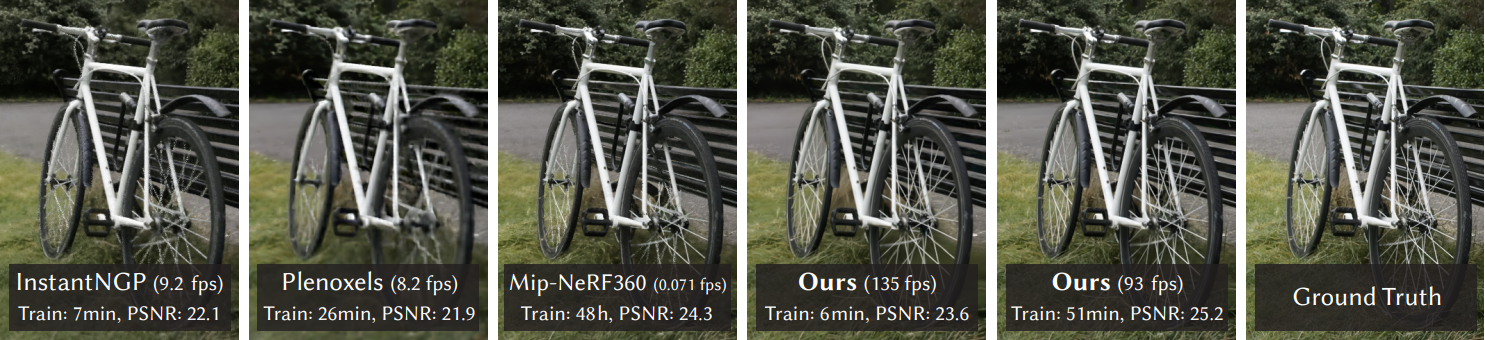
\includegraphics[width=0.92\textwidth]{images/3dgs_teaser.png}

  \vspace{0.4em}
  \begin{columns}[c]
    \begin{column}{0.32\textwidth}
      \begin{block}{\centering Real-time rendering}
        \centering \textbf{$>$90 FPS} at 1080p
      \end{block}
    \end{column}
    \begin{column}{0.32\textwidth}
      \begin{block}{\centering Fast training}
        \centering \textbf{20–40 min} (vs.\ 1–2 days for NeRF)
      \end{block}
    \end{column}
    \begin{column}{0.32\textwidth}
      \begin{block}{\centering Quality}
        \centering \textbf{Comparable} to state-of-the-art NeRF
      \end{block}
    \end{column}
  \end{columns}
\end{frame}

% ============================================================
% SLIDE 5 — The Gaussian Primitive (visual)
% ============================================================
\begin{frame}{Building Block: The 3D Gaussian "Blob"}
  \begin{columns}[c]
    \begin{column}{0.50\textwidth}
      Each Gaussian is like a \textbf{colored, transparent soap bubble}:

      \vspace{0.8em}
      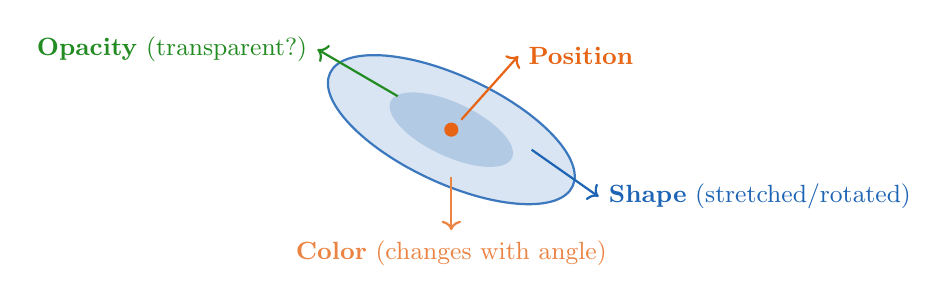
\begin{tikzpicture}[scale=0.85, every node/.style={font=\small}]
        % Gaussian ellipse
        \begin{scope}[rotate around={-25:(0,0)}]
          \fill[gaussblue!20, draw=gaussblue, thick, opacity=0.85]
            (0,0) ellipse (2.0cm and 0.8cm);
          \fill[gaussblue!50, opacity=0.5]
            (0,0) ellipse (1.0cm and 0.4cm);
        \end{scope}
        \fill[accentorange] (0,0) circle (3pt);

        % Labels with arrows
        \draw[->, accentorange, thick] (0.15,0.15) -- (1,1.1)
          node[right, accentorange] {\textbf{Position}};
        \draw[->, gaussblue, thick] (1.2,-0.3) -- (2.2,-1.0)
          node[right, gaussblue] {\textbf{Shape} (stretched/rotated)};
        \draw[->, softgreen, thick] (-0.8,0.5) -- (-2.0,1.2)
          node[left, softgreen] {\textbf{Opacity} (transparent?)};
        \draw[->, accentorange!80, thick] (0,-0.7) -- (0,-1.5)
          node[below, accentorange!80] {\textbf{Color} (changes with angle)};
      \end{tikzpicture}
    \end{column}
    \begin{column}{0.48\textwidth}
      \begin{block}{A scene = millions of blobs}
        \begin{itemize}
          \item Between \textbf{100,000 and 10 million} blobs per scene
          \item Each blob has \textbf{59 numbers} that define it completely
          \item All learned automatically from photos!
        \end{itemize}
      \end{block}

      \vspace{2em}
      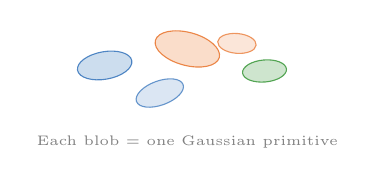
\begin{tikzpicture}[scale=0.7]
        % Mini scene with multiple gaussians
        \begin{scope}[rotate around={10:(-1.5,0.3)}]
          \fill[gaussblue!30, draw=gaussblue, opacity=0.75] (-1.5,0.3) ellipse (0.5cm and 0.25cm);
        \end{scope}
        \begin{scope}[rotate around={-15:(0.0,0.6)}]
          \fill[accentorange!30, draw=accentorange, opacity=0.75] (0.0,0.6) ellipse (0.6cm and 0.3cm);
        \end{scope}
        \begin{scope}[rotate around={5:(1.4,0.2)}]
          \fill[softgreen!30, draw=softgreen, opacity=0.75] (1.4,0.2) ellipse (0.4cm and 0.2cm);
        \end{scope}
        \begin{scope}[rotate around={20:(-0.5,-0.2)}]
          \fill[gaussblue!25, draw=gaussblue, opacity=0.65] (-0.5,-0.2) ellipse (0.45cm and 0.22cm);
        \end{scope}
        \begin{scope}[rotate around={-5:(0.9,0.7)}]
          \fill[accentorange!25, draw=accentorange, opacity=0.65] (0.9,0.7) ellipse (0.35cm and 0.18cm);
        \end{scope}
        \node[below, font=\tiny, gray] at (0,-0.8) {Each blob = one Gaussian primitive};
      \end{tikzpicture}
    \end{column}
  \end{columns}
\end{frame}

% ============================================================
% SLIDE 6 — Shape: Scale + Rotate
% ============================================================
\begin{frame}{Blob Shape: Stretch and Rotate}
  \centering
  \textbf{Every blob can be any shape and orientation — like kneading clay}

  \vspace{0.8em}
  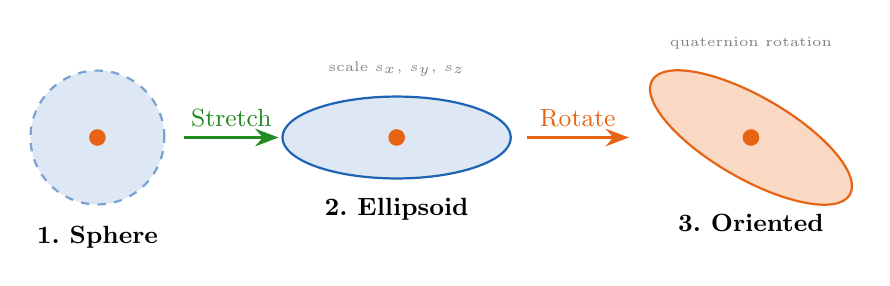
\begin{tikzpicture}[scale=1.0, every node/.style={font=\small}]
  % ── Step 1: Sphere ──────────────────────────────────────────────
\node[above, font=\tiny, gray] at (-6,0) {start};
\fill[gaussblue!15]  (-6,0) circle (0.85cm);
\draw[gaussblue!60, dashed, thick] (-6,0) circle (0.85cm);
\fill[accentorange]  (-6,0) circle (3pt);
\node[below=1.0cm, font=\small] at (-6,0) {\textbf{1.~Sphere}};

% ── Arrow 1: Stretch ────────────────────────────────────────────
\draw[-{Stealth}, softgreen, very thick]
(-4.9, 0) -- (-3.7, 0)
node[midway, above, font=\small, softgreen] {Stretch};

% ── Step 2: Ellipsoid ───────────────────────────────────────────
\node[above=0.65cm, font=\tiny, gray] at (-2.2,0)
{scale $s_x,\,s_y,\,s_z$};
\fill[gaussblue!15, draw=gaussblue, thick]
(-2.2,0) ellipse (1.45cm and 0.52cm);
\fill[accentorange] (-2.2,0) circle (3pt);
\node[below=0.65cm, font=\small] at (-2.2,0) {\textbf{2.~Ellipsoid}};

% ── Arrow 2: Rotate ─────────────────────────────────────────────
\draw[-{Stealth}, accentorange, very thick]
(-0.55, 0) -- (0.75, 0)
node[midway, above, font=\small, accentorange] {Rotate};

% ── Step 3: Oriented (rotated ellipse) ──────────────────────────
\node[above=1.0cm, font=\tiny, gray] at (2.3,0)
{quaternion rotation};
\begin{scope}[shift={(2.3,0)}, rotate=-30]
	\fill[accentorange!25, draw=accentorange, thick]
	(0,0) ellipse (1.45cm and 0.52cm);
\end{scope}
\fill[accentorange] (2.3,0) circle (3pt);
\node[below=0.85cm, font=\small] at (2.3,0) {\textbf{3.~Oriented}};

  \end{tikzpicture}

  \vspace{0.8em}
  \begin{columns}[c]
    \begin{column}{0.5\textwidth}
      \begin{exampleblock}{Why this is clever}
        Rotation \& scale are stored separately, so the optimizer can freely
        adjust them without breaking math constraints.
      \end{exampleblock}
    \end{column}
    \begin{column}{0.48\textwidth}
      \centering
      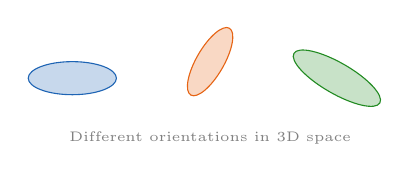
\begin{tikzpicture}[scale=0.7]
        % Three different blobs
        \begin{scope}[rotate=0]
          \fill[gaussblue!25, draw=gaussblue] (-2.5,0) ellipse (0.8cm and 0.3cm);
        \end{scope}
        \begin{scope}[rotate around={60:(0,0.3)}]
          \fill[accentorange!25, draw=accentorange] (0,0.3) ellipse (0.7cm and 0.25cm);
        \end{scope}
        \begin{scope}[rotate around={-30:(2.3,0)}]
          \fill[softgreen!25, draw=softgreen] (2.3,0) ellipse (0.9cm and 0.28cm);
        \end{scope}
        \node[below, font=\tiny, gray] at (0,-0.8) {Different orientations in 3D space};
      \end{tikzpicture}
    \end{column}
  \end{columns}
\end{frame}

% ============================================================
% SLIDE 7 — Spherical Harmonics (visual only)
% ============================================================
\begin{frame}{Color that Changes with the Viewing Angle}
  \begin{columns}[c]
    \begin{column}{0.42\textwidth}
      \textbf{Real surfaces look different depending on where you look from:}

      \vspace{0.5em}
      \begin{itemize}
        \item A metallic ball has highlights
        \item Glass reflects the environment
        \item Wet surfaces are shiny from some angles
      \end{itemize}

      \vspace{0.5em}
      \textbf{Spherical Harmonics} capture this effect — like a flexible
      colour function on a sphere. Each blob stores \textbf{48 colour values}
      that together encode how colour changes with direction.
    \end{column}
    \begin{column}{0.56\textwidth}
      \centering
      % Visual: increasing complexity of SH lobes
      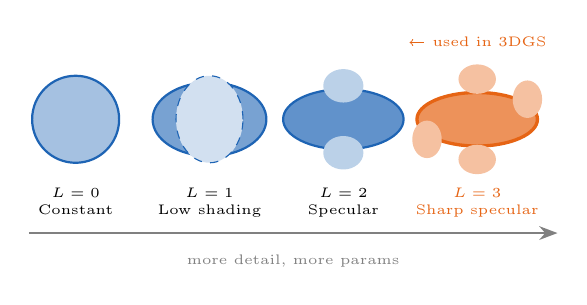
\begin{tikzpicture}[scale=0.85, node distance=0.4cm]
        % L=0 (constant - just a colored disk)
        \fill[gaussblue!40, draw=gaussblue, thick] (-4.5, 0) circle (0.65cm);
        \node[below=0.75cm, font=\tiny, align=center] at (-4.5,0)
          {$L=0$\\Constant};

        % L=1 (directional - slightly distorted)
        \fill[gaussblue!60, draw=gaussblue, thick]
          (-2.5, 0) ellipse (0.85cm and 0.55cm);
        \fill[gaussblue!20, draw=gaussblue, dashed]
          (-2.5, 0) ellipse (0.5cm and 0.65cm);
        \node[below=0.75cm, font=\tiny, align=center] at (-2.5,0)
          {$L=1$\\Low shading};

        % L=2 (quadratic - more lobes)
        \fill[gaussblue!70, draw=gaussblue, thick]
          (-0.5, 0) ellipse (0.9cm and 0.45cm);
        \fill[gaussblue!30] (-0.5, 0.5) ellipse (0.3cm and 0.25cm);
        \fill[gaussblue!30] (-0.5, -0.5) ellipse (0.3cm and 0.25cm);
        \node[below=0.75cm, font=\tiny, align=center] at (-0.5,0)
          {$L=2$\\Specular};

        % L=3 (sharp - many lobes)
        \fill[accentorange!70, draw=accentorange, very thick]
          (1.5, 0) ellipse (0.9cm and 0.4cm);
        \fill[accentorange!40] (1.5, 0.6) ellipse (0.28cm and 0.22cm);
        \fill[accentorange!40] (1.5, -0.6) ellipse (0.28cm and 0.22cm);
        \fill[accentorange!40] (2.25, 0.3) ellipse (0.22cm and 0.28cm);
        \fill[accentorange!40] (0.75, -0.3) ellipse (0.22cm and 0.28cm);
        \node[below=0.75cm, font=\tiny, align=center, accentorange] at (1.5,0)
          {\textbf{$L=3$}\\Sharp specular};
        \node[above=0.8cm, font=\tiny, accentorange] at (1.5,0) {← used in 3DGS};

        % Arrow below
        \draw[-{Stealth}, thick, gray]
          (-5.2,-1.7) -- (2.7,-1.7)
          node[midway, below=0.15cm, font=\tiny] {more detail, more params};
      \end{tikzpicture}

      \vspace{0.4em}
      \begin{alertblock}{\centering Training trick}
        \centering Start simple ($L=0$), unlock complexity every 1000 steps.
      \end{alertblock}
    \end{column}
  \end{columns}
\end{frame}

% ============================================================
% SLIDE 7b — Spherical Harmonics: nodal lines
% ============================================================
\begin{frame}{Spherical Harmonics: Nodal Lines}
  \centering
  \textbf{Each degree adds more angular detail — the nodal lines show where color changes sign}

  \vspace{0.5em}
  \animategraphics[loop, autoplay, width=0.75\textwidth]{12}{images/gifs/nodal_frames/frame-}{000}{065}

  \vspace{0.4em}
  \begin{exampleblock}{\centering What you see}
    \centering The lobes grow and rotate as higher SH degrees are added —
    exactly how 3DGS encodes view-dependent color per Gaussian.
  \end{exampleblock}
\end{frame}

% ============================================================
% SLIDE 8 — Rendering: Splatting
% ============================================================
\begin{frame}{Rendering: Squashing Blobs onto the Screen}
  \centering
  \textbf{To make an image, each 3D blob is "splatted" (projected) onto the camera plane}

  \vspace{0.6em}
  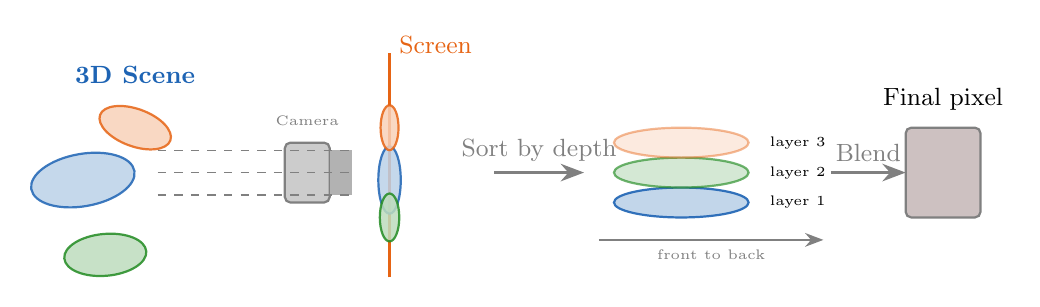
\begin{tikzpicture}[scale=0.95, every node/.style={font=\small}]

    % 3D space label
    \node[font=\small, gaussblue] at (-4.8, 2.2) {\textbf{3D Scene}};

    % 3D Gaussians
    \foreach \cx/\cy/\rx/\ry/\rot/\col in {
        -5.5/0.8/0.7/0.35/10/gaussblue,
        -4.8/1.5/0.5/0.25/-20/accentorange,
        -5.2/-0.2/0.55/0.28/5/softgreen}{
      \begin{scope}[rotate around={\rot:(\cx,\cy)}]
        \fill[\col!30, draw=\col, thick, opacity=0.85]
          (\cx,\cy) ellipse (\rx cm and \ry cm);
      \end{scope}
    }

    % Camera
    \fill[gray!40, draw=gray, thick, rounded corners=2pt]
      (-2.8, 0.5) rectangle (-2.2, 1.3);
    \fill[gray!60] (-2.2, 0.6) rectangle (-1.9, 1.2);
    \node[above, font=\tiny, gray] at (-2.5, 1.4) {Camera};

    % Projection lines
    \foreach \y in {0.6, 0.9, 1.2}{
      \draw[gray, dashed] (-4.5,\y) -- (-1.9,\y);
    }

    % Screen plane
    \draw[accentorange, thick] (-1.4,-0.5) -- (-1.4,2.5);
    \node[right, font=\small, accentorange] at (-1.4, 2.6) {Screen};

    % 2D splatted Gaussians on screen
    \fill[gaussblue!30, draw=gaussblue, thick, opacity=0.85]
      (-1.4,0.8) ellipse (0.15cm and 0.45cm);
    \fill[accentorange!30, draw=accentorange, thick, opacity=0.85]
      (-1.4,1.5) ellipse (0.12cm and 0.3cm);
    \fill[softgreen!30, draw=softgreen, thick, opacity=0.85]
      (-1.4,0.3) ellipse (0.13cm and 0.32cm);

    % Arrow to process
    \draw[-{Stealth}, very thick, gray] (0.0,0.9) -- (1.2,0.9)
      node[midway, above, font=\small] {Sort by depth};

    % Stack of layers
    \foreach \i/\col/\op in {1/gaussblue/0.9, 2/softgreen/0.65, 3/accentorange/0.45}{
      \fill[\col!30, draw=\col, thick, opacity=\op]
        (2.5,{0.4*\i+0.1}) ellipse (0.9cm and 0.2cm);
      \node[right=1.0cm, font=\tiny] at (2.5,{0.4*\i+0.1})
        {layer \i};
    }

    % Arrow to pixel
    \draw[-{Stealth}, very thick, gray] (4.5,0.9) -- (5.5,0.9)
      node[midway, above, font=\small] {Blend};

    % Final pixel
    \fill[gaussblue!50!accentorange!40, draw=gray, thick, rounded corners=2pt]
      (5.5, 0.3) rectangle (6.5, 1.5);
    \node[above, font=\small] at (6.0, 1.6) {Final pixel};

    % Depth label
    \draw[-{Stealth}, thick, gray] (1.4, 0.0) -- (4.4, 0.0)
      node[midway, below, font=\tiny] {front to back};

  \end{tikzpicture}

  \vspace{0.3em}
  \begin{exampleblock}{\centering Key insight}
    \centering
    Unlike NeRF (which shoots rays), 3DGS \textbf{rasterizes} blobs directly
    onto the screen — exactly like how game engines render triangles. This is why it's so fast.
  \end{exampleblock}
\end{frame}

% ============================================================
% SLIDE 9 — Alpha Compositing (simplified)
% ============================================================
\begin{frame}{Layering Colours: Like Transparent Paint}
  \begin{columns}[c]
    \begin{column}{0.48\textwidth}
      \textbf{Think of it like stacking transparent acetates:}

      \vspace{0.5em}
      \begin{enumerate}
        \item Sort Gaussians \textbf{front to back}
        \item Each layer contributes some colour and blocks some light behind it
        \item Stop when the pixel is fully covered
      \end{enumerate}

      \vspace{0.5em}
      \begin{block}{Final pixel colour}
        \[
          \mathbf{C} = \sum_{i} \underbrace{\mathbf{c}_i}_{\text{colour}}
            \cdot \underbrace{\alpha_i}_{\text{opacity}}
            \cdot \underbrace{T_i}_{\text{how much light reaches layer }i}
        \]
      \end{block}
    \end{column}
    \begin{column}{0.50\textwidth}
      \centering
      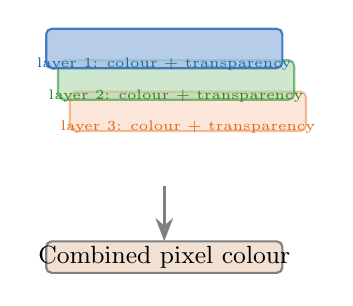
\begin{tikzpicture}[scale=1.0, every node/.style={font=\small}]
        % Acetate analogy
        \foreach \i/\col/\opacity in {
            3/accentorange/0.4,
            2/softgreen/0.55,
            1/gaussblue/0.8}{
          \fill[\col!40, draw=\col, thick, opacity=\opacity, rounded corners=2pt]
            ({0.15*\i-0.15},{-0.4*\i+1.5}) rectangle ({3+0.15*\i-0.15},{0.5-0.4*\i+1.5});
          \node[font=\tiny, \col] at ({1.5+0.15*\i-0.15},{0.05-0.4*\i+1.5})
            {layer \i: colour + transparency};
        }
        % Arrow down
        \draw[-{Stealth}, very thick, gray] (1.5,-0.4) -- (1.5,-1.1);
        % Result
        \fill[gaussblue!30!softgreen!20!accentorange!20, draw=gray, thick, rounded corners=2pt]
          (0,-1.5) rectangle (3,-1.1);
        \node[font=\small, align=center] at (1.5,-1.3) {Combined pixel colour};
      \end{tikzpicture}

      \vspace{0.4em}
      \begin{exampleblock}{\centering Same math as NeRF}
        \centering This blending is \emph{mathematically equivalent}
        to NeRF's ray integrals — just computed much faster.
      \end{exampleblock}
    \end{column}
  \end{columns}
\end{frame}

% ============================================================
% SLIDE 10 — Training: Adaptive Density Control
% ============================================================
\begin{frame}{Training: The Scene Builds Itself}
  \begin{columns}[c]
    \begin{column}{0.46\textwidth}
      \textbf{Start with a sparse point cloud, then refine:}

      \vspace{0.6em}
      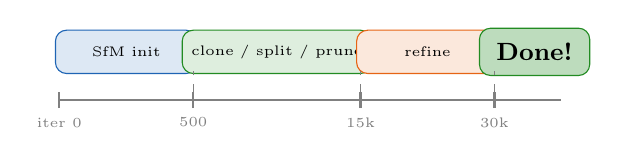
\begin{tikzpicture}[scale=0.85, every node/.style={font=\small}]
          % ── Timeline bar ────────────────────────────────────────────────
        \draw[thick, gray] (0,0) -- (7.5,0);
        
        % Tick marks + labels
        \foreach \x/\lbl in {0/iter~0, 2.0/500, 4.5/15k, 6.5/30k}{
        	\draw[gray, thick] (\x,-0.12) -- (\x,0.12);
        	\node[below, font=\tiny, gray] at (\x,-0.12) {\lbl};
        }
        
        % ── Box 1: SfM init  (iter 0 → 500)  center ≈ 1.0 ──────────────
        \node[draw=gaussblue, fill=gaussblue!15, rounded corners,
        font=\tiny, minimum width=1.8cm, minimum height=0.55cm]
        at (1.0, 0.72) {SfM init};
        
        % ── Box 2: clone/split/prune (500 → 15k)  center ≈ 3.25 ─────────
        \node[draw=softgreen, fill=softgreen!15, rounded corners,
        font=\tiny, minimum width=2.3cm, minimum height=0.55cm]
        at (3.25, 0.72) {clone / split / prune};
        
        % ── Box 3: refine  (15k → 30k)  center ≈ 5.5 ───────────────────
        \node[draw=accentorange, fill=accentorange!15, rounded corners,
        font=\tiny, minimum width=1.8cm, minimum height=0.55cm]
        at (5.5, 0.72) {refine};
        
        % ── Box 4: Done!  (after 30k)  center ≈ 7.1 ────────────────────
        \node[draw=softgreen, fill=softgreen!30, rounded corners,
        font=\small, minimum width=1.4cm, minimum height=0.6cm]
        at (7.1, 0.72) {\textbf{Done!}};
        
        % ── Dashed vertical guides ───────────────────────────────────────
        \foreach \x in {2.0, 4.5, 6.5}{
        	\draw[gray, dashed, thin] (\x, 0.12) -- (\x, 0.44);
        }
      \end{tikzpicture}

      \vspace{0.5em}
      \begin{block}{Loss: rendered vs.\ real photo}
        Compare each rendered frame to the training photo. Adjust all blobs to reduce the error.
      \end{block}
    \end{column}

    \begin{column}{0.52\textwidth}
      \centering
      \textbf{Three adaptive operations every 100 iterations:}

      \vspace{0.4em}
      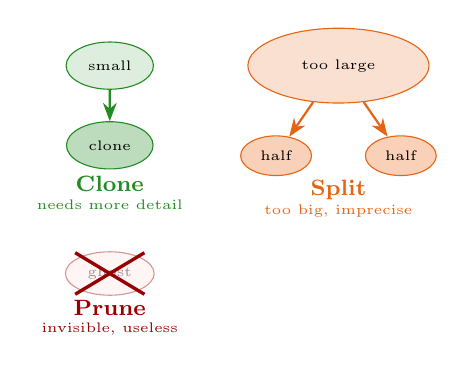
\begin{tikzpicture}[scale=0.88, every node/.style={font=\small}]
        % CLONE
        \node[draw=softgreen, fill=softgreen!15, ellipse,
              minimum width=1.1cm, minimum height=0.6cm] (sm) at (-2.0,1.9) {\tiny small};
        \node[draw=softgreen, fill=softgreen!30, ellipse,
              minimum width=1.1cm, minimum height=0.6cm] (cl) at (-2.0,0.75) {\tiny clone};
        \draw[-{Stealth}, softgreen, thick] (sm)--(cl);
        \node[font=\footnotesize, softgreen] at (-2.0,0.2) {\textbf{Clone}};
        \node[font=\tiny, softgreen] at (-2.0,-0.1) {needs more detail};

        % SPLIT
        \node[draw=accentorange, fill=accentorange!20, ellipse,
              minimum width=2.3cm, minimum height=0.95cm] (big) at (1.3,1.9) {\tiny too large};
        \node[draw=accentorange, fill=accentorange!30, ellipse,
              minimum width=0.9cm, minimum height=0.5cm] (s1) at (0.4,0.6) {\tiny half};
        \node[draw=accentorange, fill=accentorange!30, ellipse,
              minimum width=0.9cm, minimum height=0.5cm] (s2) at (2.2,0.6) {\tiny half};
        \draw[-{Stealth}, accentorange, thick] (big)--(s1);
        \draw[-{Stealth}, accentorange, thick] (big)--(s2);
        \node[font=\footnotesize, accentorange] at (1.3,0.1) {\textbf{Split}};
        \node[font=\tiny, accentorange] at (1.3,-0.2) {too big, imprecise};

        % PRUNE
        \node[draw=red!60!black, fill=red!10, ellipse,
              minimum width=0.7cm, minimum height=0.4cm,
              opacity=0.4] (ghost) at (-2.0,-1.1) {\tiny ghost};
        \draw[red!60!black, very thick] (-2.5,-0.8) -- (-1.5,-1.4);
        \draw[red!60!black, very thick] (-1.5,-0.8) -- (-2.5,-1.4);
        \node[font=\footnotesize, red!60!black] at (-2.0,-1.6) {\textbf{Prune}};
        \node[font=\tiny, red!60!black] at (-2.0,-1.9) {invisible, useless};
      \end{tikzpicture}
    \end{column}
  \end{columns}
\end{frame}

% ============================================================
% SLIDE 11 — Limitations & Future
% ============================================================
\begin{frame}{Where It Struggles \& Where It's Going}
  \begin{columns}[c]
    \begin{column}{0.5\textwidth}
      \textbf{Current limitations:}

      \vspace{0.5em}
      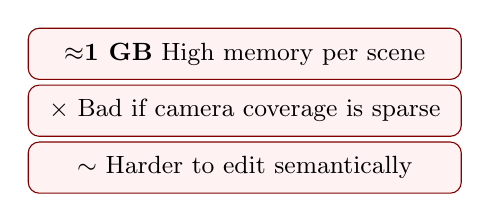
\begin{tikzpicture}[scale=0.85, every node/.style={font=\small}]
        \foreach \i/\ico/\desc in {
            0/{$\approx$1 GB}/{High memory per scene},
            1/{$\times$}/{Bad if camera coverage is sparse},
            2/{$\sim$}/{Harder to edit semantically}}{
          \node[draw=red!50!black, fill=red!5, rounded corners,
                minimum width=5.5cm, minimum height=0.65cm, align=left]
            at (0,{-\i*0.85}) {\textbf{\ico}\ \desc};
        }
      \end{tikzpicture}
    \end{column}
    \begin{column}{0.5\textwidth}
      \textbf{Exciting future directions:}

      \vspace{0.5em}
      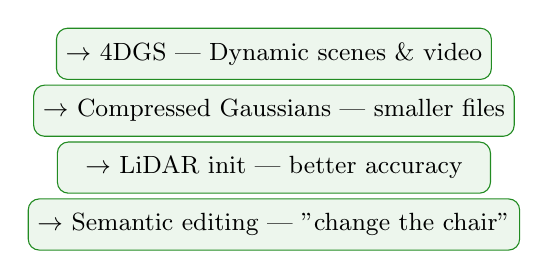
\begin{tikzpicture}[scale=0.85, every node/.style={font=\small}]
        \foreach \i/\desc in {
            0/{4DGS — Dynamic scenes \& video},
            1/{Compressed Gaussians — smaller files},
            2/{LiDAR init — better accuracy},
            3/{Semantic editing — "change the chair"}}{
          \node[draw=softgreen, fill=softgreen!8, rounded corners,
                minimum width=5.5cm, minimum height=0.65cm, align=left]
            at (0,{-\i*0.85}) {$\rightarrow$ \desc};
        }
      \end{tikzpicture}
    \end{column}
  \end{columns}
\end{frame}

% ============================================================
% SLAM SECTION — Introduction
% ============================================================
\begin{frame}{From Rendering to SLAM}
  \begin{columns}[c]
    \begin{column}{0.50\textwidth}
      \textbf{SLAM} = \alert{Simultaneous Localisation and Mapping}

      \vspace{0.6em}
      A robot (or camera) must answer two questions \textbf{at the same time}:
      \begin{enumerate}
        \item \textbf{Where am I?} (localisation)
        \item \textbf{What does the environment look like?} (mapping)
      \end{enumerate}

      \vspace{0.6em}
      \begin{block}{Classic SLAM maps}
        Point clouds · Occupancy grids · Meshes
      \end{block}

      \vspace{0.4em}
      \begin{exampleblock}{3DGS SLAM maps}
        Millions of coloured Gaussians — photorealistic \emph{and} real-time!
      \end{exampleblock}
    \end{column}
    \begin{column}{0.48\textwidth}
      \centering
      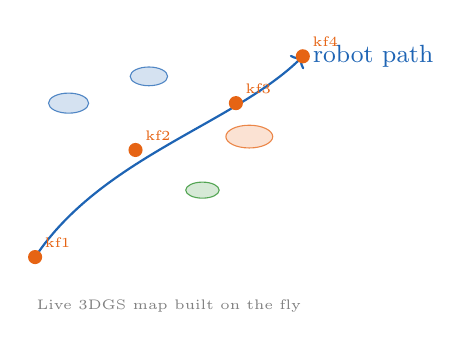
\begin{tikzpicture}[scale=0.85, every node/.style={font=\small}]
        % Robot path
        \draw[gaussblue, thick, ->] (-2,-1.5) .. controls (-1,0) and (1,0.5) .. (2,1.5)
          node[right] {robot path};
        % Keyframes
        \foreach \pt/\n in {(-2,-1.5)/1, (-0.5,0.1)/2, (1,0.8)/3, (2,1.5)/4}{
          \fill[accentorange] \pt circle (3pt);
          \node[above right, font=\tiny, accentorange] at \pt {kf\n};
        }
        % Gaussians scattered around
        \foreach \cx/\cy/\rx/\ry/\col in {
            -1.5/0.8/0.30/0.15/gaussblue,
            0.5/-0.5/0.25/0.12/softgreen,
            1.2/0.3/0.35/0.17/accentorange,
            -0.3/1.2/0.28/0.14/gaussblue}{
          \fill[\col!25, draw=\col, opacity=0.75] (\cx,\cy) ellipse (\rx cm and \ry cm);
        }
        \node[below, font=\tiny, gray] at (0,-2.0) {Live 3DGS map built on the fly};
      \end{tikzpicture}
    \end{column}
  \end{columns}
\end{frame}

% ============================================================
% SLAM — How 3DGS enables SLAM
% ============================================================
\begin{frame}{3DGS-SLAM: Key Systems}
  \begin{columns}[c]
    \begin{column}{0.52\textwidth}
      \textbf{How 3DGS integrates with SLAM:}

      \vspace{0.5em}
      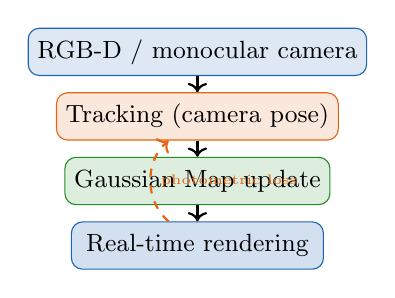
\begin{tikzpicture}[scale=0.82, every node/.style={font=\small},
                          box/.style={draw, rounded corners, minimum width=3.2cm,
                                      minimum height=0.6cm, align=center}]
        \node[box, fill=gaussblue!15, draw=gaussblue]  (cam) at (0,3.0) {RGB-D / monocular camera};
        \node[box, fill=accentorange!15, draw=accentorange] (track) at (0,2.0) {Tracking (camera pose)};
        \node[box, fill=softgreen!15, draw=softgreen]  (map)  at (0,1.0) {Gaussian Map update};
        \node[box, fill=gaussblue!20, draw=gaussblue]  (ren)  at (0,0.0) {Real-time rendering};

        \draw[->, thick] (cam)   -- (track);
        \draw[->, thick] (track) -- (map);
        \draw[->, thick] (map)   -- (ren);
        \draw[->, thick, dashed, accentorange] (ren) to[bend left=50]
          node[right, font=\tiny] {photometric loss} (track);
      \end{tikzpicture}
    \end{column}
    \begin{column}{0.46\textwidth}
      \textbf{Notable 3DGS-SLAM systems:}

      \vspace{0.4em}
      \begin{itemize}
        \item \textbf{SplaTAM} (2024) — first real-time 3DGS SLAM\\
              {\small RGB-D input, silhouette-guided densification}
        \item \textbf{Gaussian-SLAM} — online scene reconstruction\\
              {\small runs at $>$10 fps on a single GPU}
        \item \textbf{MonoGaussian} — monocular camera only\\
              {\small depth estimated from monocular cues}
      \end{itemize}

      \vspace{0.4em}
      \begin{alertblock}{\centering Advantage over classic SLAM}
        \centering The map is \textbf{photorealistic} — useful for AR, robotics, and loop closure.
      \end{alertblock}
    \end{column}
  \end{columns}
\end{frame}

% ============================================================
% SLAM — Tracking with Gaussians
% ============================================================
\begin{frame}{Pose Estimation via Photometric Loss}
  \centering
  \textbf{Camera pose is found by minimising the difference between rendered and real frames}

  \vspace{0.5em}
  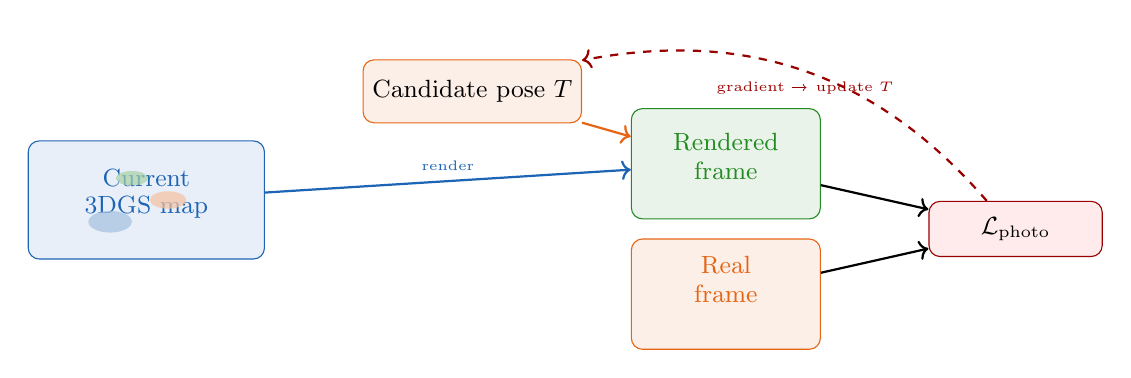
\begin{tikzpicture}[scale=0.92, every node/.style={font=\small}]
    % Current 3DGS map
    \node[draw=gaussblue, fill=gaussblue!10, rounded corners,
          minimum width=3.0cm, minimum height=1.5cm] (map) at (-4.5, 0) {};
    \node[font=\small, gaussblue] at (-4.5, 0.3) {Current};
    \node[font=\small, gaussblue] at (-4.5,-0.1) {3DGS map};
    % Gaussians inside
    \fill[gaussblue!40, opacity=0.7] (-5.0,-0.3) ellipse (0.3cm and 0.15cm);
    \fill[accentorange!40, opacity=0.7] (-4.2, 0.0) ellipse (0.25cm and 0.12cm);
    \fill[softgreen!40, opacity=0.7] (-4.7, 0.3) ellipse (0.22cm and 0.10cm);

    % Candidate pose
    \node[draw=accentorange, fill=accentorange!10, rounded corners,
          minimum width=2.2cm, minimum height=0.8cm] (pose) at (0, 1.5) {Candidate pose $T$};

    % Rendered frame
    \node[draw=softgreen, fill=softgreen!10, rounded corners,
          minimum width=2.4cm, minimum height=1.4cm] (ren) at (3.5, 0.5) {};
    \node[font=\small, softgreen] at (3.5, 0.8) {Rendered};
    \node[font=\small, softgreen] at (3.5, 0.4) {frame};

    % Real frame
    \node[draw=accentorange, fill=accentorange!10, rounded corners,
          minimum width=2.4cm, minimum height=1.4cm] (real) at (3.5,-1.3) {};
    \node[font=\small, accentorange] at (3.5,-0.9) {Real};
    \node[font=\small, accentorange] at (3.5,-1.3) {frame};

    % Loss
    \node[draw=red!60!black, fill=red!8, rounded corners,
          minimum width=2.2cm, minimum height=0.7cm] (loss) at (7.5, -0.4) {$\mathcal{L}_\text{photo}$};

    % Arrows
    \draw[->, thick, gaussblue] (map)  -- node[above, font=\tiny]{render} (ren);
    \draw[->, thick, accentorange] (pose) -- (ren);
    \draw[->, thick] (ren)  -- (loss);
    \draw[->, thick] (real) -- (loss);
    \draw[->, thick, red!60!black, dashed] (loss) to[bend right=30]
      node[below, font=\tiny]{gradient → update $T$} (pose);
  \end{tikzpicture}

  \vspace{0.3em}
  \begin{exampleblock}{\centering Result}
    \centering The pose $T$ is optimised iteratively — camera tracks the scene \textbf{and} the Gaussian map is updated online.
  \end{exampleblock}
\end{frame}

% ============================================================
% DEMO — Live 3DGS result
% ============================================================
\begin{frame}{Live Result: 3DGS in Action}
  \centering
  \textbf{Real scan reconstructed with 3D Gaussian Splatting}

  \vspace{0.6em}
  \movie[width=0.82\textwidth, height=0.55\textheight, autostart, loop,
         poster, showcontrols]{%
    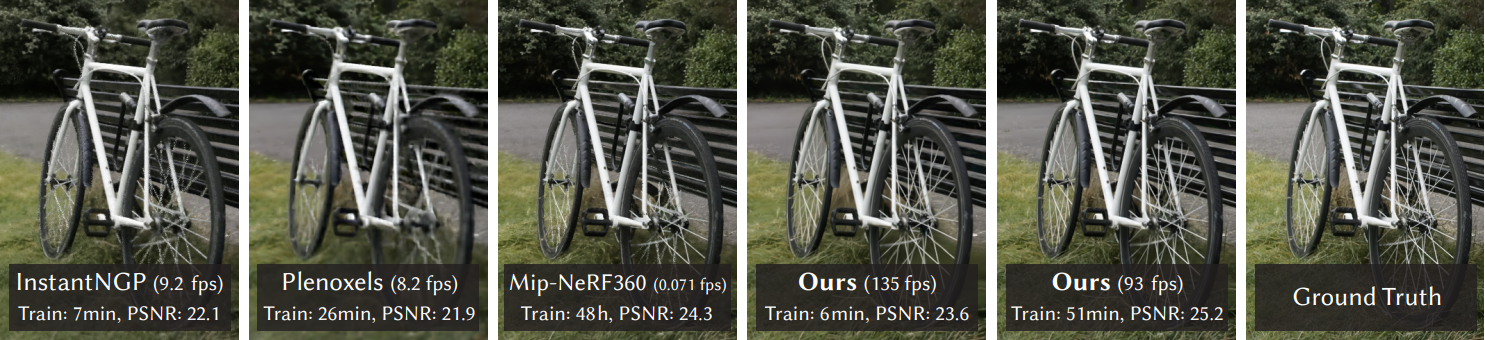
\includegraphics[width=0.82\textwidth]{images/3dgs_teaser.png}%
  }{video/3dgs_demo.mp4}

  \vspace{0.4em}
  {\small\color{gray} Click to play — requires Adobe Acrobat or a compatible PDF viewer}
\end{frame}

% ============================================================
% SLIDE 18 — SLAM Optimisations
% ============================================================
\begin{frame}{System Optimisations for Real-Time SLAM}
  \begin{itemize}
    \item \textbf{Memory \& Keyframing:}\\ Optimising the map at 60 FPS would crash the GPU. \alert{Solution:} The system selects \textbf{Keyframes} (when the camera moves significantly) and optimises a small "sliding window". Transparent or oversized Gaussians are aggressively pruned.
    \vspace{0.5em}
    \item \textbf{Smart Initialization:}\\ To prevent mid-air "floaters", new Gaussians are only spawned where the rendered silhouette detects a physical "hole" in the map.
    \vspace{0.5em}
    \item \textbf{Fixing Trajectory Drift:}\\ As the camera travels, tiny tracking errors accumulate. \alert{Solution:} Upon recognizing a visited area (\textbf{Loop Closure}), the system runs a \textbf{Global Bundle Adjustment} to realign historical poses and millions of Gaussian parameters simultaneously.
  \end{itemize}
\end{frame}

% ============================================================
% SLIDE 19 — Performance Trade-offs
% ============================================================
\begin{frame}{Performance Analysis: NeRF vs. 3DGS SLAM}
  \begin{table}
    \centering
    \renewcommand{\arraystretch}{1.4}
    \begin{tabular}{l c c}
      \toprule
      \textbf{Metric} & \textbf{NeRF-SLAM} & \textbf{3DGS-SLAM} \\
      \midrule
      \textbf{Tracking \& Mapping} & 1 -- 5 FPS & 10 -- 30+ FPS \\
      \textbf{Rendering Speed} & $< 10$ FPS & $> 90$ FPS \\
      \textbf{VRAM (Room Scale)} & $< 1$ GB & 2 -- 6+ GB \\
      \textbf{Primary Bottleneck} & Compute Bound & Memory Bound \\
      \bottomrule
    \end{tabular}
  \end{table}
  \vspace{0.5em}
  \begin{itemize}
    \item \textbf{NeRF:} Highly memory efficient, but too slow for real-time AR/VR.
    \item \textbf{3DGS:} Unbeatable speed and visual quality, but severe memory bottleneck (can exceed 24 GB for large outdoor maps).
  \end{itemize}
\end{frame}


\begin{frame}{Why is it so fast? Tile-Based Rasterisation}
  NeRF is slow because it shoots a ray for every pixel and queries a heavy Neural Network hundreds of times along that ray (\textbf{Volumetric Ray Marching}).
  
  \vspace{1em}
  3DGS skips the neural network entirely during rendering:
  \begin{enumerate}
    \item \textbf{Project:} It flattens the 3D ellipsoids onto the 2D screen (Splatting).
    \item \textbf{Divide \& Sort:} It splits the screen into $16 \times 16$ pixel tiles and uses an ultra-fast GPU Radix Sort to order the Gaussians from front-to-back.
    \item \textbf{Blend:} It rapidly blends the colours and opacities (Alpha-compositing).
  \end{enumerate}
  
  \vspace{0.5em}
  \centering \alert{$\Rightarrow$ This native GPU pipeline is why 3DGS achieves $>90$ FPS.}
\end{frame}

% ============================================================
% SLIDE 20 — SLAM Evaluation Metrics
% ============================================================
\begin{frame}{How do we evaluate SLAM?}
  \begin{itemize}
    \item \textbf{Tracking Accuracy (Where am I?)}
    \begin{itemize}
      \item \textbf{ATE (Absolute Trajectory Error):} Measures the physical deviation (in cm) between the estimated camera path and the true ground-truth path.
    \end{itemize}
    \vspace{1em}
    \item \textbf{Mapping Fidelity (What does the world look like?)}
    \begin{itemize}
      \item \textbf{PSNR \& SSIM:} Measure pixel-perfect accuracy and structural similarity of the rendered map against real photos.
      \item \textbf{LPIPS:} Measures how accurate the map looks to \textit{human perception} using deep neural networks.
    \end{itemize}
  \end{itemize}
\end{frame}

% ============================================================
% SLIDE 21 — Limitations & Future Work
% ============================================================
\begin{frame}{Limitations \& Active Research}
  \begin{itemize}
    \item \textbf{Dynamic Scenes}\\ 3DGS assumes a static world. Moving people or cars leave "ghost" trails.
    \begin{itemize}
      \item \alert{Solution:} Emerging \textbf{4D Gaussian Splatting (4DGS)} adds time-dependent velocity to Gaussians.
    \end{itemize}
    \vspace{1em}
    \item \textbf{Storage Footprint}\\ A single room can take $\sim$1 GB of disk space.
    \begin{itemize}
      \item \alert{Solution:} Aggressive compression techniques like \textbf{Vector Quantization}, \textbf{Attribute Pruning} (dropping high-order Spherical Harmonics), and \textbf{Entropy Coding} can reduce file sizes by over 50\%.
    \end{itemize}
  \end{itemize}
\end{frame}

% ============================================================
% SLIDE 22 — Conclusion
% ============================================================
\begin{frame}{Conclusion}
  \begin{itemize}
    \item \textbf{Paradigm Shift:}\\ 3DGS represents a fundamental shift from \alert{Compute-bound} (NeRF) to \alert{Memory-bound} SLAM.
    \vspace{0.8em}
    \item \textbf{Unification:}\\ It successfully unifies high-fidelity photorealistic reconstruction with real-time camera tracking ($>90$ FPS rendering).
    \vspace{0.8em}
    \item \textbf{The Verdict:}\\ 3DGS is the definitive future for interactive AR/VR and robotics, provided that upcoming research can solve its VRAM and dynamic scene limitations.
  \end{itemize}
\end{frame}

% ============================================================
% SLIDE FINAL — Q&A
% ============================================================
\begin{frame}[standout]
  \centering
  \LARGE \textbf{Questions?}\\[1em]
  \normalsize
  Jaime Hernández · Yauheni Yatsevich\\
  Universidad de Alicante, March 2026
\end{frame}

\end{document}
